\chapter{Fundamentação Teórica}
\label{chap:fundamentacao_teorica}

A proposta deste trabalho visa unificar informações das \textit{features} radiômicas e \textit{features} profundas oriundas de uma rede neural convolucional e, por conseguinte, propor uma arquitetura de \textit{self-attention} para identificar características discriminantes afim de obter resultados relevantes na classificação de cardiomiopatia hipertrófica. Os fundamentados os seguintes conceitos: análise radiômica, extração de \textit{features} profundas e redes \textit{transformers}.

%--------------------------------------------------------
\section{Ressonância Magnética em Cardiomiopatia}

A ressonância magnética (RM) está se tornando o principal método de imagem para avaliar a fisiologia e a função na doença cardíaca congênita. A RM possui funções que normalmente são obtidas por ecocardiografia, tendo como exemplo a velocidade média em um vaso, mas também apresenta características muito especiais como calcular a velocidade em um voxel de um milímetro em qualquer lugar no espaço tridimensional do vaso.
Usando a tecnologia atual de RM, os investigadores podem obter percepções únicas sobre a função ventricular, por exemplo, deformação ventricular regional in vivo e movimento da parede e mecânica dos fluidos, por exemplo, visualização in vivo de perfis de velocidade além de aumentar a precisão de medidas padrão aceitas pela fisiologia ou função ventricular, por exemplo, débito cardíaco, volumes ventriculares e massa. Devido ao rápido avanço da tecnologia, muitas técnicas de RM são experimentais ou ainda estão em fase de desenvolvimento clínico; no entanto, há muitas técnicas que são clinicamente úteis, por exemplo, medição do volume ventricular em pacientes com tamanho ventricular esquerdo limítrofe. Como muitas das técnicas experimentais atuais serão, sem dúvida, empregadas na prática clínica no futuro, os médicos devem estar cientes de todo o espectro de capacidades da RM \cite{fogelAssessmentCardiacFunction2000}.

Em muitos cenários clínicos, as limitações técnicas da ecocardiografia e a expressão fenotípica heterogênea tornaram tal avaliação difícil, e a RM cardíaca emergiu como uma modalidade de imagem complementar útil para complementar a ecocardiografia transtorácica de rotina. A RM cardíaca é única em sua alta resolução espacial e temporal com excelente contraste entre o pool sanguíneo e o miocárdio, sem limitação de janela de imagem ou plano de imagem.
A heterogeneidade fenotípica da miocardiopatia hipertrófica é bem reconhecida pela dificuldade em sua identificação. Isto se complica ainda mais pois nem todos os pacientes com hipertrofia ventricular esquerda têm CMH, enquanto uma fisiopatologia semelhante à CMH com obstrução dinâmica do trato de saída do ventrículo esquerdo pode ser observada sem hipertrofia do ventrículo esquerdo, em um subgrupo de pacientes com anormalidades na válvula mitral e/ou no músculo papilar.

A CMH é uma doença heterogênea com expressão morfológica complexa que requer uma caracterização precisa da doença para um planejamento terapêutico ótimo e estratificação de risco. A RM cardíaca emergiu como um complemento útil para esses propósitos. Com a incorporação crescente de imagem multimodal na avaliação clínica da CMH, nosso entendimento sobre a importância de diferenças morfológicas sutis continuará a crescer, e pesquisas adicionais definirão novos marcadores prognósticos e melhorarão as estratégias de tratamento atuais\cite{toCardiacMagneticResonance2011c}.


%Diferentemente de outras áreas que utilizam e geram majoritariamente dados textuais, a Medicina também faz uso massivo de imagens para composição de seus diagnósticos. Independentemente do propósito da imagem, nos últimos anos esses equipamentos também evoluíram e se tornaram mais precisos, proporcionando um volume maior de dados e imagens, que exigem uma maior capacidade de armazenamento (ISSA; BYERS; DAKSHANAMURTHY, 2014).

%Algumas modalidades médicas como a Ressonância Magnética Cardíaca (RMC) e a Tomografia Computadorizada (TC) são exemplos de exames que podem gerar objetos tridimensionais (3D) de estruturas específicas do corpo humano a partir de dezenas de fatias (BANKMAN; MORCOVESCU, 2002). Um outro aspecto que também desafia a comunidade médica é a fadiga visual, percebida quando o especialista realiza a análise contínua de muitas imagens.


% Expostos esses fatores, torna-se relevante o desenvolvimento de métodos inteligentes para armazenamento e recuperação dessas imagens médicas que são geradas diariamente. Nesse sentindo, os sistemas de Diagnóstico Auxiliado por Computador (Computer-Aided Diagnosis - CAD) têm o propósito de apoiar especialistas médicos em seus diagnósticos, uma vez que o tempo demandado para analisar essas imagens tem se tornado cada vez maior (DATTA et al., 2008).

%--------------------------------------------------------
\section{Análise Radiômica}

A análise radiômica é um campo de pesquisa em rápida evolução, preocupado com a extração de informações quantitativas, incluindo padrões complexos que são difíceis de reconhecer ou quantificar pelo olho humano dentro de imagens médicas, características estas chamadas  de\textit{features} radiômicas. As \textit{features} radiômicas podem capturar características de tecidos e lesões, como forma e heterogeneidade, e podem, sozinhas ou em combinação com dados demográficos, histológicos, genômicos ou proteômicos, ser usadas para a resolução de problemas clínicos. O objetivo desta seção é fornecer uma introdução ao campo, cobrindo o fluxo de trabalho básico da análise radiômica: cálculo e seleção de características, redução de dimensionalidade e processamento de dados \cite{mayerhoeferIntroductionRadiomics2020}.

Embora \textit{features} radiômica individuais podem se correlacionar com dados genômicos ou dados clínicos, o impacto da análise radiômica se torna mais relevante a medida que mais informações são por ela extraídas. Tipicamente centenas de \textit{features}, uma fração das do total extraído, contribuem para identificação de uma doença específica e é processada usando técnicas de aprendizado de máquina.

As \textit{features} radiômicas podem ser subdivididas em estatísticas, incluindo as baseadas em histograma e textura; modelo; transformação; e forma. A extração pode ser dada em regiões de interesse de 2-dimensões (2D) e 3-dimensões (3D).

%--------------------------------------------------------
\subsection{\textit{Features} por Histograma}

Os descritores estatísticos mais simples são baseados no histograma global de níveis de cinza e incluem média de nível de cinza, máximo, mínimo, variância e percentis. Como essas características são baseadas em análises de pixel único ou voxel único (3D), elas são chamadas de características de primeira ordem. Algumas \textit{features} mais sofisticadas incluem assimetria e curtose que descrevem a forma da distribuição de intensidade dos dados: a assimetria reflete a assimetria da curva de distribuição dos dados para a esquerda (assimetria negativa, abaixo da média) ou direita (assimetria positiva, acima da média), enquanto a curtose reflete a caudalidade de uma distribuição de dados em relação a uma distribuição gaussiana devido a \textit{outliers}. Outras \textit{features} incluem histograma entrópico e uniformidade (também chamado de energia).

%--------------------------------------------------------
\subsection{\textit{Features} de Textura}

Uma abordagem simples para a descrição de textura radiômica é a análise do gradiente absoluto, que reflete o grau ou a abruptidade das flutuações de intensidade de nível de cinza em uma imagem. Para dois \textit{pixels} ou \textit{voxels} adjacentes, o gradiente é o máximo possível quando um for preto e o outro branco, enquanto se ambos os \textit{pixels} forem pretos (ou ambos forem brancos) o gradiente nessa localidade é zero. Similares as \textit{features} por histograma, as \textit{features} por gradiente incluem média, variância, assimetria e curtose (Fig. \ref{fig:fig001}).

\captionsetup{justification=centering}
\begin{figure}[htbp]
    \centering
    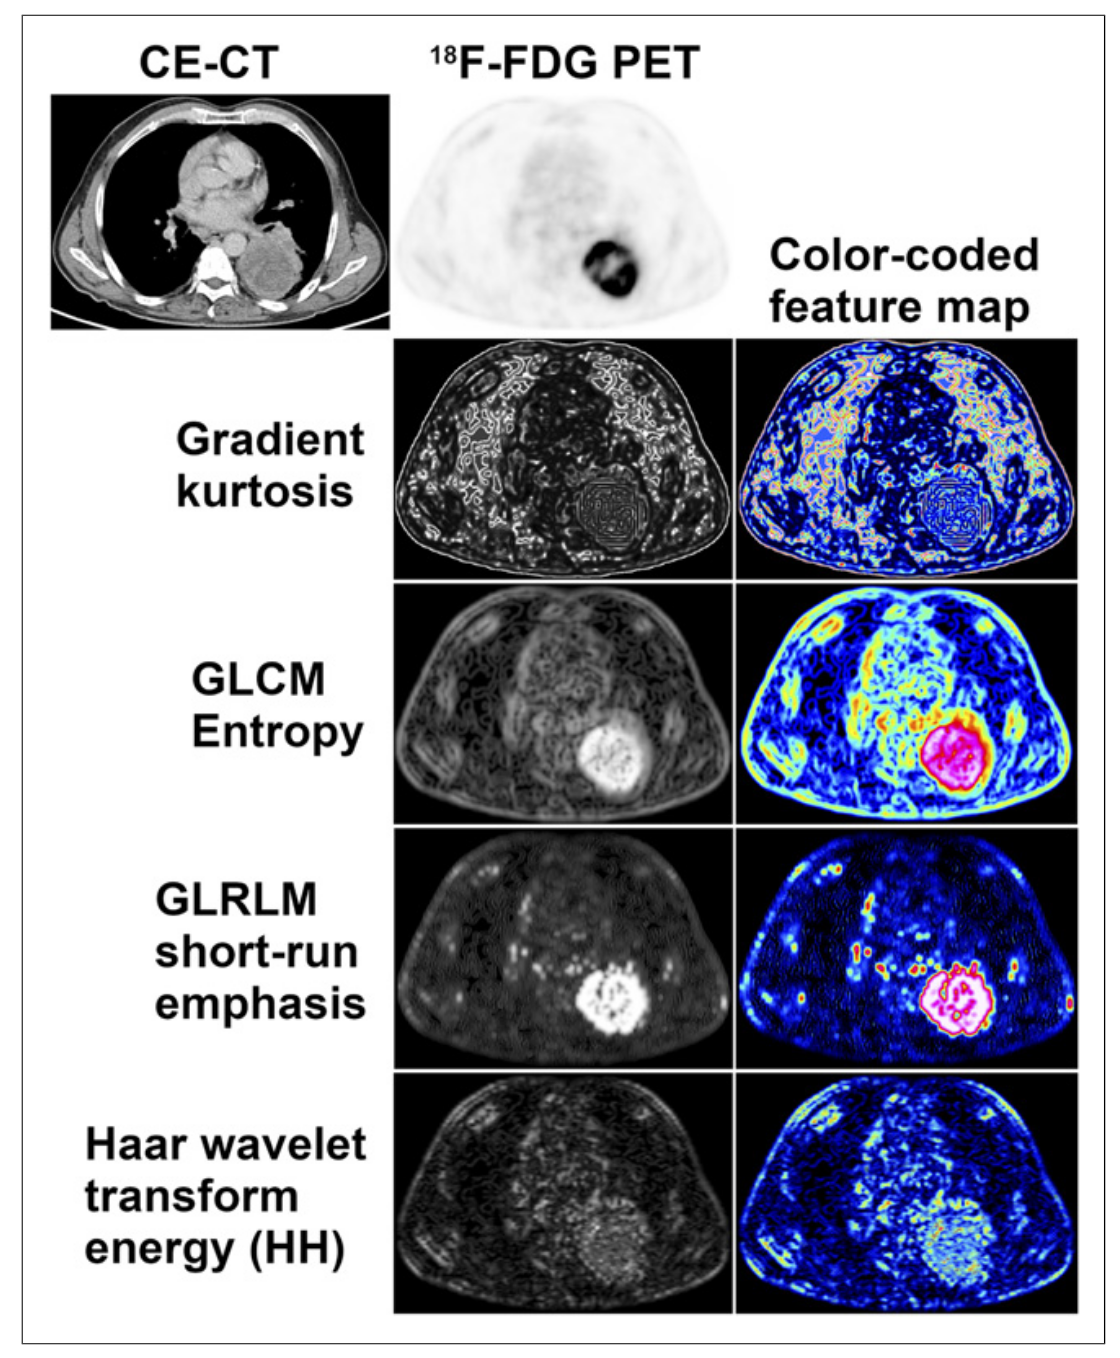
\includegraphics[width=0.6\textwidth]{figures/fig001.png}
    \caption{Exemplos de análise radiômica.}
    \label{fig:fig001}
\end{figure}

 \textit{GLCM}. A matriz de coocorrência de níveis de cinza, do termo \gls{GLCM} é um histograma em níveis de cinza de segunda ordem. O GLCM captura relações espaciais entre pares de \textit{pixels} ou \textit{voxels} com níveis de níveis de cinza pré-definidos, em diferentes direções (horizontal, vertical ou diagonal para análise 2D, 13 direções para 3D) e com uma distância pré-definida entre os \textit{pixels} ou \textit{voxels} (Fig. \ref{fig:fig002}). As \textit{features} de GLCM incluem entropia (Fig. \ref{fig:fig002}), uma medida de  compostas por uma medida da inomogeneidade ou aleatoriedade dos níveis de cinza, momento angular de segunda ordem (também chamado de uniformidade ou energia), que reflete a homogeneidade ou ordem dos níveis de cinza e contraste, que enfatiza as diferenças nos níveis de cinza entre \textit{pixels} ou \textit{voxels} pertencentes a um par de \textit{pixel} ou \textit{voxel}.

 \textit{GLRLM}. A matriz de comprimento de corrida de níveis de cinza, do termo 
 \textit{Gray-Level Run-length Matrix} (GLRLM) fornece informações sobre a distribuição espacial das sequências de \textit{pixels} consecutivos com os mesmos níveis de cinza, em uma ou mais direções, em 2 ou 3 dimensões. As características da GLRLM incluem fração, que avalia a porcentagem de \textit{pixels} ou \textit{voxels} dentro da região de interesse que fazem parte das sequências e, portanto, reflete a granulosidade. 

\textit{GLSZM}. A matriz de zona do tamanho dos níveis de cinza, do termo \textit{Gray-Level Size Zone Matrix} (GLSZM) é baseada no mesmo princípio do GLRLM porém aqui, contagens do número de grupos (chamados zonas) de pixels ou voxels vizinhos interconectados com o mesmo nível de cinza formam a base para a matriz (Fig. \ref{fig:fig002}. Uma textura mais homogênea resultará em uma matriz mais ampla e plana. A GLSZM não é calculada para diferentes direções, mas pode ser calculada para diferentes distâncias de pixels ou voxels que definem a vizinhança. As \textit{features} da GLSZM podem ser calculadas em 2 dimensões (8 pixels vizinhos) ou 3 dimensões (26 voxels vizinhos) e, seguindo as definições da GLRLM, incluem fração (porcentagem de pixels ou voxels que fazem parte das zonas), ênfase em zonas grandes e pequenas, entre outras.

\begin{figure}[htbp]
    \centering
    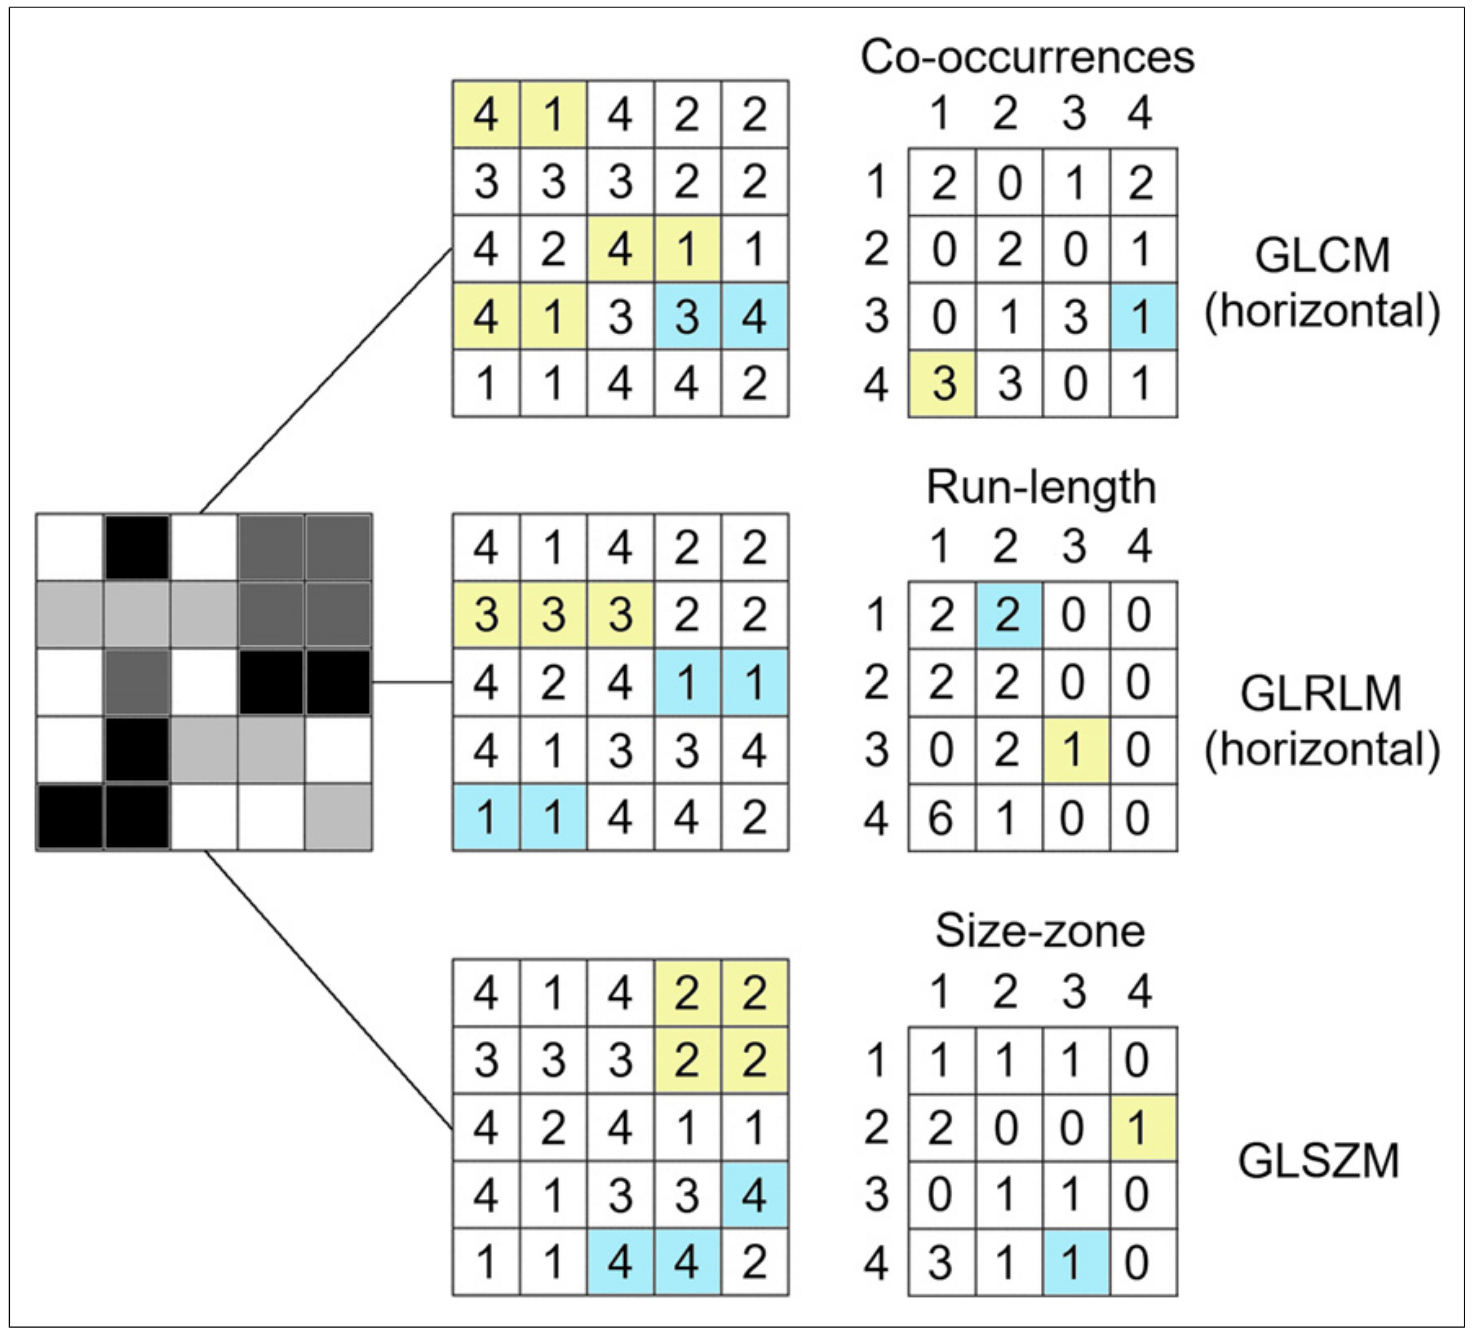
\includegraphics[width=0.6\textwidth]{figures/fig002.png}
    \caption{Exemplos de análise radiômica.}
    \label{fig:fig002}
\end{figure}

%--------------------------------------------------------
\subsection{\textit{Features} de Modelo}

As análises baseadas em modelos visam interpretar \textit{features} em níveis de cinza espaciais para caracterizar objetos ou formas. Um modelo parametrizado de geração de textura é calculado e ajustado à região de interesse (ROI), e seus parâmetros estimados são utilizados como \textit{features} radiômicas. O modelo autorregressivo é um exemplo de abordagem baseada em modelo e baseia-se na ideia de que o nível de cinza de um pixel é uma soma ponderada dos níveis de cinza de 4 pixels vizinhos. Além disso, $\sigma$, a qual carrega informações sobre a variância do erro de previsão mínimo, mede a regularidade da textura. A análise fractal também produz recursos que podem ser usados na análise radiômica, em particular a dimensão fractal, que reflete a taxa de adição de detalhe estrutural com o aumento da magnificação, escala ou resolução e, portanto, serve como uma medida de complexidade. A lacunaridade, um recurso que mede a falta de invariância rotacional ou translacional, reflete a inomogeneidade \cite{mayerhoeferIntroductionRadiomics2020}.

%--------------------------------------------------------
\subsection{\textit{Features} de Transformação}
Métodos Baseados em Transformadas, incluindo transformadas de \textit{Fourier}, \textit{Gabor} e de \textit{wavelets} de \textit{Haar}, analisam padrões de níveis de cinza em um espaço diferente. A transformada discreta de \textit{wavelet} de \textit{Haar}, por exemplo, analisa o conteúdo da frequência de uma imagem em diferentes escalas. A decomposição por \textit{wavelets} de uma imagem é possível aplicando um par de filtros espelhados em quadratura, um filtro de passa-alta e um de passa-baixa. Embora o filtro de passa-alta destaque as mudanças no nível de cinza e, assim, enfatize detalhes da imagem, o filtro de passa-baixa suaviza a imagem em termos de nível de cinza, removendo detalhes da imagem. Após a decomposição do sinal, um conjunto de canais de frequência orientados espacialmente está disponível, o qual é usado para descrever a variabilidade local da imagem. As energias dentro dos canais de frequência são então usadas como \textit{features}. A filtragem de passa-alta em ambas as direções (Fig. \ref{fig:fig001}) captura detalhes diagonais, a filtragem de passa-alta seguida por filtragem de passa-baixa captura bordas verticais, a filtragem de passa-baixa seguida por filtragem de passa-alta captura bordas horizontais, e a filtragem de passa-baixa em ambas as direções captura as frequências mais baixas, em diferentes escalas. Notavelmente, a transformação por \textit{wavelets} pode ser usada não apenas para a geração de \textit{features} radiômicas, mas também para segmentação de imagens ou como um passo de pré-processamento para análise de textura \cite{mayerhoeferIntroductionRadiomics2020}.

%--------------------------------------------------------
\section{Extração de Features Profundas}
Para extrair \textit{features} profundas das imagens de RM, foi empregada a arquitetura pré-treinada de uma rede \textit{ResNet50}. As redes \textit{ResNet50} ficaram muito conhecidas ao fim do ano de 2015 por vencer diversas competições em visão computacional, includindo 1º lugar na competição de classificação de imagens \textit{ILSVRC} 2015. As redes \textit{ResNet}, do termo \textit{Residual Networks}, inovaram na em sua época trazendo uma forma de treinar modelos de maior profundidade, chegando a mais de 100 camadas, com resultados superiores à outros modelos convolucionais competitivos, como o \textit{VGG19}, sem sofrer os sintomas comum a estas redes muito profundas que seriam o de \textit{overfitting} e a saturação/ausência dos gradientes em tempo de treino. Os autores da \textit{ResNet} sugeriram o uso de saltos de conexão entre as camadas da rede (Fig. \ref{fig:fig003}) afim de manter os gradientes relevantes e controlados entre uma camada e outra.  A \textit{ResNet50} é um modelo de rede neural convolucional profunda de 50 camadas que compreende muitos blocos residuais. Cada bloco contém módulos de convolução e uma conexão de salto que transfere a informação do bloco anterior para o próximo bloco. A conexão de salto ajuda a reter a informação semântica mais baixa aprendida nas camadas anteriores, que de outra forma se tornaria abstrata devido à conexão de longa cadeia. A conexão de salto também evita que o gradiente desapareça nas camadas mais profundas, fornecendo um caminho alternativo para a retropropagação. A informação da conexão de salto é adicionada à informação calculada em cada bloco \cite{heDeepResidualLearning2015}.

Várias abordagens de sucesso aplicaram redes convolucionais para extrair características genéricas para tarefas de recuperação de imagens e obtiveram resultados promissores. Elas utilizam principalmente o poder das \textit{features} locais para gerar uma representação de uma imagem genérica baseada em redes convolucionais pré-treinadas. As representações das camadas finais da rede convolucional são utilizadas para capturar \textit{features} semânticas para o fim de nível de categoria à classificação que o modelo se dispõe \cite{alzubiContentbasedImageRetrieval2017b}.

\begin{figure}[htbp]
    \centering
    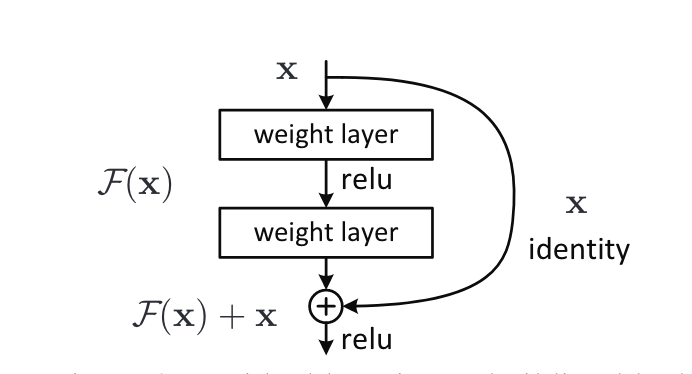
\includegraphics[width=0.6\textwidth]{figures/fig003.png}
    \caption{Aprendizado Residual: bloco}
    \label{fig:fig003}
\end{figure}

%--------------------------------------------------------
\section{Arquitetura Transformers}

A arquitetura \textit{Transformers} é uma estado da arte que se propôs a resolver as limitações das arquiteturas recorrentes e sua dificuldade em manter as relações entre pontos dentre as camadas recorrentes além das restrições vinculadas ao custo de computação sequencial. O modelo de arquitetura \textit{transformers} se utiliza do mecanismo de atenção e este se tornou parte integral de modelos de modelagem de sequências e transdução convincentes em várias tarefas, permitindo a modelagem de dependências sem considerar a distância entre elas nas sequências de entrada ou saída. Os \textit{transformers} como arquitetura descarta o uso de módulos de recorrência e se utiliza inteiramente do mecanismo de atenção para capturar as dependências globais entre entrada e saída. Os \textit{transformers} também são responsáveis por um ganho significante em paralelismo em sua execução \cite{vaswaniAttentionAllYou2023}.

\begin{figure}[htbp]
    \centering
    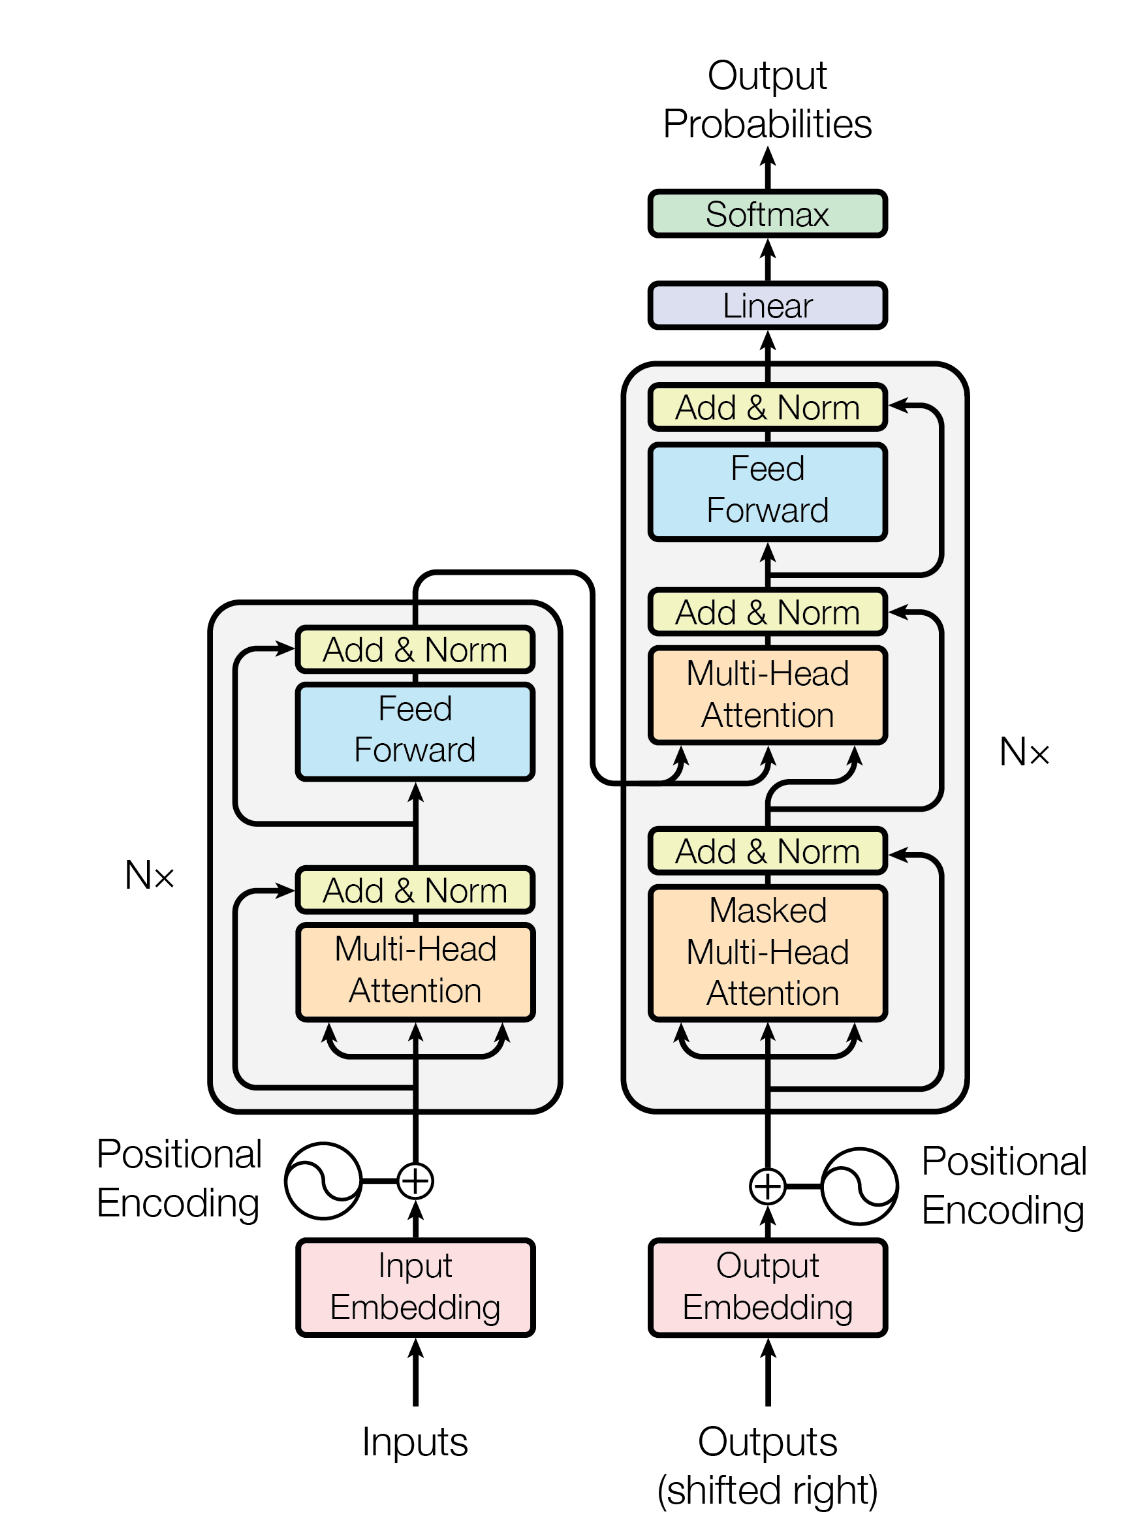
\includegraphics[width=0.6\textwidth]{figures/fig004.png}
    \caption{Arquitetura do \textit{Transformers}}
    \label{fig:fig004}
\end{figure}

O \textit{transformers} é composto por um \textit{Encoder} e um \textit{Decoder}, respectivamente o bloco da esquerda e direita \ref{fig:fig004}. Em ambos os \textit{Encoder} e \textit{Decoder}, tem-se como bloco cerne da rede o de atenção multi-cabeças. O mecanismo de atenção pode ser descrito mapeando uma \textit{query} e um par de chave e valor, onde a \textit{query}, chave e valor são todos vetores de saída. A saída é computada como uma soma ponderada dos valores onde o peso destinado a cada valor é computado por uma função de compatibilidade da query com a chave correspondente.

\begin{figure}[htbp]
    \centering
    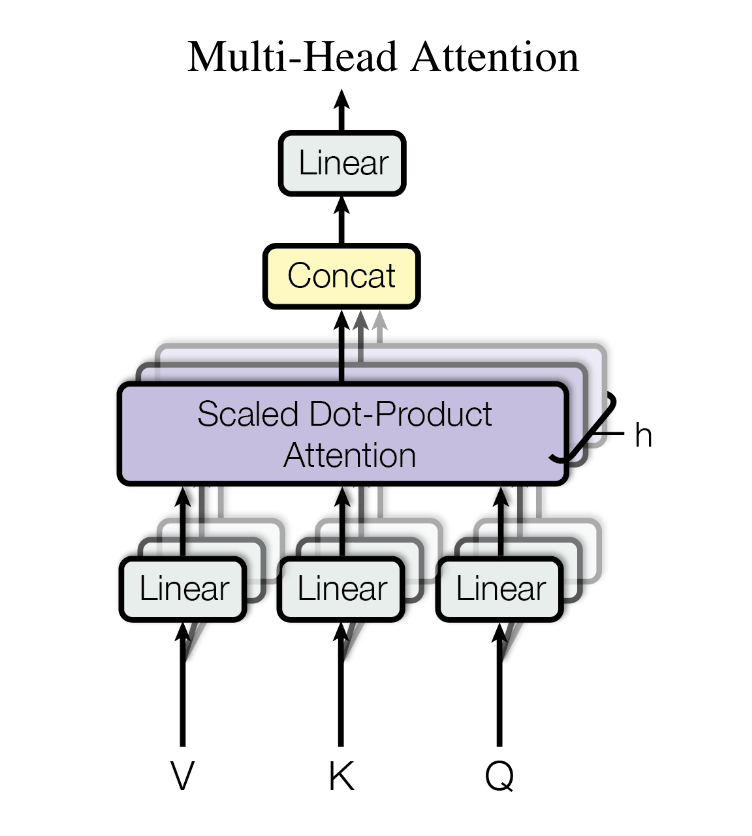
\includegraphics[width=0.6\textwidth]{figures/fig005.png}
    \caption{Arquitetura do \textit{Transformers}}
    \label{fig:fig005}
\end{figure}

O mecanismo de atenção é particularmente chamado de "Atenção de Produto Escalar Dimensionado" (Fig. \ref{fig:fig005}). A entrada consiste em consultas e chaves de dimensão $d_{k}$, e valores de dimensão $d_{v}$. É calculado os produtos escalares da consulta com todas as chaves e dividido cada um por $\sqrt{d_{k}}$. Em seguida, aplica-se uma função \textit{softmax} para obter os pesos sobre os valores. Na prática, é calculada a função de atenção em um conjunto de consultas simultaneamente, agrupadas em uma matriz $Q$. As chaves e os valores também são agrupados em matrizes $K$ e $V$. Calculamos a matriz de saídas como:

\begin{equation}
\text{Attention}(Q, K, V) = \text{softmax}\left(\frac{QK^T}{\sqrt{d_k}}\right)V
\label{eq:attention}
\end{equation}

Dos vários pontos de vantagem do mecanismo de atenção, pode-se citar: o total de poder computacional por camada, o total de computação que pode ser paralelizada e o já mencionado que seria relação de dependência entre dados que se encontram muito distantes um do outro, como também distâncias que necessitam ser percorridas frente e para trás na rede para identificar tais relações. Como benefício adicional, o mecanismo de atenção pode gerar modelos mais interpretáveis. Não apenas as cabeças de atenção individuais claramente aprendem a executar diferentes tarefas, muitas parecem exibir comportamentos relacionados à estrutura sintática e semântica das frases, no caso da aplicação em \textit{tokens} oriundos de textos.

%--------------------------------------------------------
\section{Considerações Finais do Capitulo}
\label{subsec:rcond_cap_3}

Os métodos de avaliação de cardiomiopatias, tanto via análise radiômicas por extração de textura quanto por aprendizado profundo obtiveram êxitos em análise de imagens médicas. Mesmo sabendo que estas técnicas de \textit{Machine Learning}, utilizando estes dados de textura podem ser insuficientes em capturar a complexidade e diversidade de informações a cerca do ventrículo como também pode ser afetada pela qualidade da imagem. Métodos pode aprendizado profundo podem aprender automaticamente semânticas de alto nível e informações representativas de imagens de RM sem necessidade de \textit{features} extraídas manualmente.
Métodos de aprendizado profundo tem obtido ótimos resultados em diagnósticos, segmentação, estadiamento e prognósticos. Todavia, o mesmo tem suas limitações como limitação dos dados, desafio geral na área médica, \textit{overfitting} e pouca interpretabilidade.

Dadas as vantagens e limitações discutidas, este trabalho tem como proposta a fusão de uma arquitetura de aprendizado profundo baseada no mecanismo de atenção que integras \textit{features} radiômicas e profundas para a identificação de cardiomiopatia. A arquitetura proposta é composta por: extração de \textit{features} radiômicas e profundas; redução de dimensionalidade para que ambas possuam tamanhos similares, redução estar utilizando \textit{F-Test}; concatenação das \textit{features}; aplicação do mecanismo de atenção e classificação binária do resultado. O esquemático pode ser conferido na Fig. \ref{fig:fig011-01}.

\begin{figure}[htbp]
    \centering
    \caption{Arquitetura Proposta}
    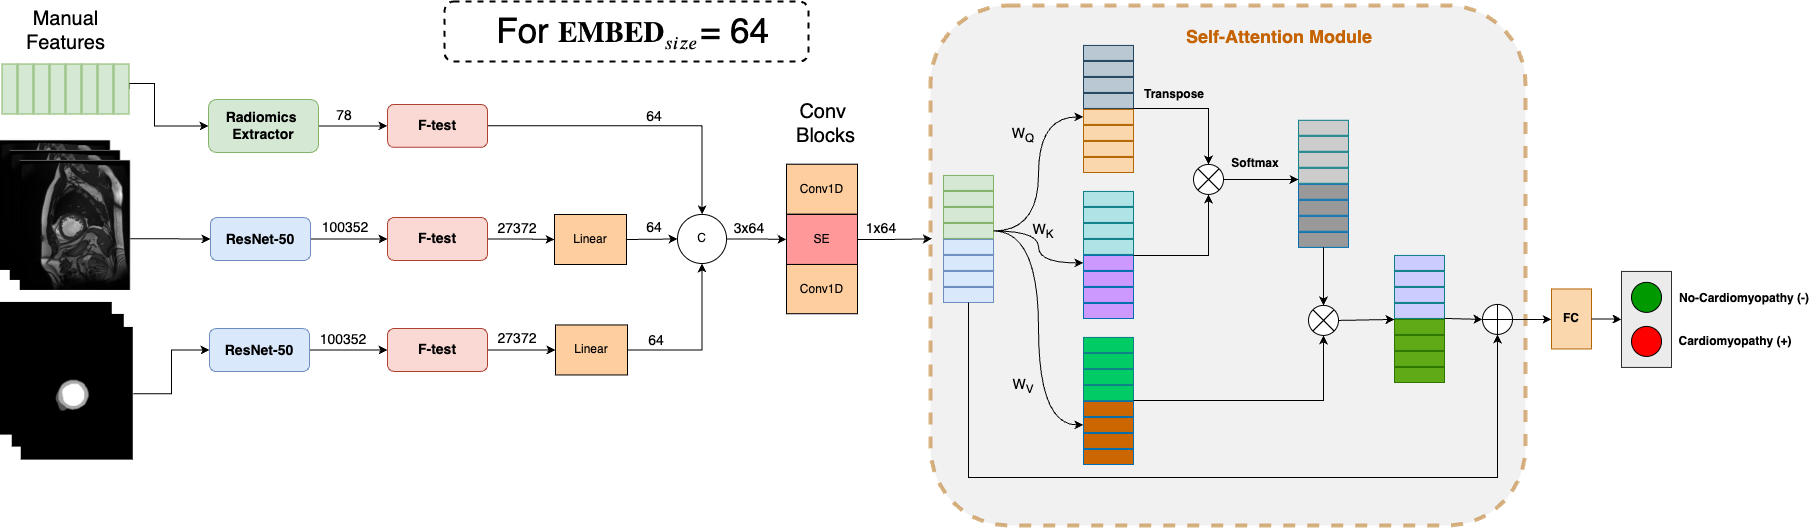
\includegraphics[width=1\textwidth]{figures/fig011.png}
    \caption*{Fonte: Autor}
    \label{fig:fig011-01}
\end{figure}

Com esta abordagem, acredita-se que será aproveitada a riqueza de informações contidas nas imagens de RM e ajustadas de forma adaptativa a importância destas \textit{features}. A fusão das \textit{features} radiômicas manuais e as \textit{features} profundas, devem melhorar as habilidades de expressividade e generalização do modelo. 